\documentclass{../../../kin_math}

\header{Elijah Kin}{Homework 7}{AMSC660}
\headrule

\begin{document}

\begin{questions}
  \question Do \textbf{matrix completion} in two ways:
  \begin{enumerate}
    \item Use the low-rank factorization model $A \approx XY^\top$ and the objective function of the form
    \begin{equation*}
      F(X, Y) = \frac{1}{2} \lVert P_\Omega(A - XY^\top) \rVert_F^2 + \frac{\lambda}{2} (\lVert X \rVert_F^2 + \lVert Y \rVert_F^2).
    \end{equation*}
    Try values of $\lambda$ 0.1, 1, and 10, and $\textsf{rank}(X) = \textsf{rank}(Y) = k$, $k = 1, 2, \dots, 7$. Find $X$ and $Y$ using alternating iteration
    \begin{equation}
      \label{eq:iter}
      X^{m + 1} = \arg \min_X F(X, Y^m),
    \end{equation}
    \begin{equation}
      Y^{m + 1} = \arg \min_Y F(X^{m + 1}, Y).
    \end{equation}
    Each of these steps can be further decomposed into a collection of small linear least squares problems. For example, at each substep of (\ref{eq:iter}), we solve the linear least squares problem to compute the row $i$ of $X$:
    \begin{equation}
      \textbf{x}_i^\top = \arg \min_\textbf{x} \frac{1}{2} \left\lVert \textbf{x}^\top Y_{\Omega_i}^\top - a_{\Omega_i} \right\rVert_2^2 + \frac{\lambda}{2} \lVert \textbf{x} \rVert^2,
    \end{equation}
    where $\Omega_i \coloneqq \{j \mid (i, j) \in \Omega\}$, $Y_{\Omega_i}^\top$ is the set of columns of $Y^\top$ with indices in $\Omega_i$, and $a_{\Omega_i}$ is the set of known entries of $A$ in its row $i$. A similar problem can be set up for each column of $Y$. Work out solutions to these problems in a manner similar to the one in Sections 5.3.1 and 5.3.2 of \texttt{LinearAlgebra.pdf} except that there will be no constraint requiring the entries to be positive. Implement the resulting algorithm. Comment on how the value of $\lambda$ and the choice of rank affects the result. Which values of the rank and $\lambda$ seem the most reasonable to you? You can judge by your own row.
    \begin{solution}
      We will update the row $i$ of $X$ by solving the linear system
      \begin{equation*}
        (Y_{\Omega_i}^\top Y_{\Omega_i} + \lambda I) \textbf{x}_i = Y_{\Omega_i}^\top a_{\Omega_i}
      \end{equation*}
      and likewise for row $j$ of $Y$,
      \begin{equation*}
        (X_{\Omega_j}^\top X_{\Omega_j} + \lambda I) \textbf{y}_j = X_{\Omega_j}^\top a_{\Omega_j}
      \end{equation*}
      suggesting the code \href{https://github.com/elijahkin/school/blob/main/umd/amsc660/hw7/hw7.ipynb}{here}. We find that smaller values of $\lambda$ achieve smaller values of $\lVert P_\Omega(A - M) \rVert_2$; on other hand, the larger the value of $k$, the smaller the value of $\lVert P_\Omega(A - M) \rVert_2$. Of the values of $\lambda$ and $k$ suggested, $\lambda = 0.1$ and $k = 7$ produces the most reasonable result with respect to the norm over the known values of $A$.
    \end{solution}
    \item Use the approach of penalizing the nuclear norm in Section 6.3 of \texttt{LinearAlgebra.pdf} and the iteration
    \begin{equation*}
      M^{j + 1} = S_\lambda(M^j + P_\Omega(A - M^j))
    \end{equation*}
    Experiment with different values of $\lambda$.
    \begin{solution}
      We implement the method of penalizing the nuclear norm via the code \href{https://github.com/elijahkin/school/blob/main/umd/amsc660/hw7/hw7.ipynb}{here}. We find that the smaller the value of $\lambda$, the smaller the norm $\lVert P_\Omega(A - M) \rVert_2$.
    \end{solution}
  \end{enumerate}
  Compare these two approaches for matrix completion. Which one gives more sensible results? Which one is easier to use? Which one do you find more efficient?
  \begin{solution}
    The method of penalizing the nuclear yields both better results and was much easier to implement and reason about.
  \end{solution}

  \question Adding the nuclear norm into the objective function for the matrix completion problem promotes low  rank. The reason is that the level set of $\lVert A \rVert_* = a$ tend to have corners, and the minimizers of the objective function including the nuclear norm penalty term tend to lie at these corners. Check experimentally that nuclear norm level set for a $2 \times 2$ matrix
  \begin{equation*}
    A = \begin{bmatrix} 0.5 & x \\ y & z \end{bmatrix}
  \end{equation*}
  have corners at points where $\det A = 0$. Proceed as follows. Let $a = 1$. Set a grid for the values of $z$:
  \begin{equation*}
    z \in \{-0.4, -0.3, -0.2, -0.1, 0, 0.1, 0.2, 0.3, 0.4\}
  \end{equation*}
  For each grid value of $z$ plot two curves on the same figure. Curve 1: the zero level set of the determinant of $A$. Curve 2: the level set $\lVert A \rVert_* = a$. Note at which points these curves intersect.
  \begin{solution}
    We plot the curves for all specified values of $z$ via \href{https://github.com/elijahkin/school/blob/main/umd/amsc660/hw7/hw7.ipynb}{this code}. We plot the case of $z = 0.1$ below.
    \begin{center}
      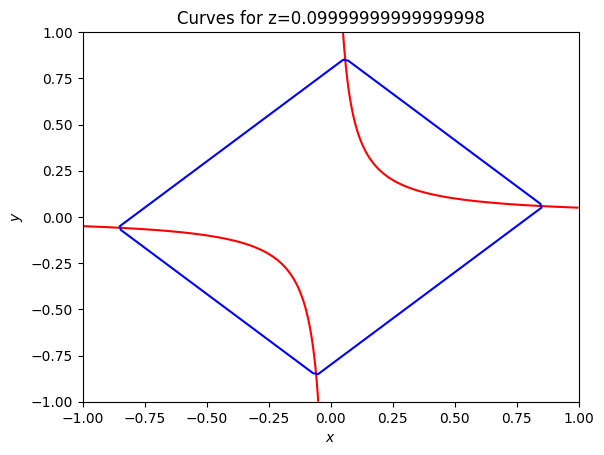
\includegraphics[scale=0.7]{curves.png}
    \end{center}
    Note that the points of intersection are at the corners of the level set $\lVert A \rVert_* = 1$. This observation holds for the other specified values of $z$ as well.
  \end{solution}

  \question Let $A$ be a symmetric positive definite matrix and let $\{p_0, \dots, p_{n - 1}\}$ be a set of vectors such that $p_j^\top A p_k = 0$ for all $j \neq k$, $0 \leq j, k \leq n - 1$. We say that this set of vectors is \emph{conjugate} with respect to the matrix $A$. Prove that this set of vectors must be linearly independent.
  \begin{solution}
    Let $\{p_0, \dots, p_{n - 1}\}$ be conjugate, so that $p_j^\top A p_k = 0$ for all $j \neq k$, and toward a contradiction, suppose $\{p_0, \dots, p_{n - 1}\}$ is linearly dependent.

    Then there exist coefficients $c_0, \dots, c_{n - 1}$ not all zero such that
    \begin{equation}
      \label{eq:lindep}
      c_0 p_0 + \dots + c_{n - 1} p_{n - 1} = \vec{0}.
    \end{equation}
    In particular, we can choose $k$ such that $c_k \neq 0$. Then left multiplying (\ref{eq:lindep}) by $p_k^\top A$, on the right-hand side we see that $p_k^\top A \vec{0} = 0$, but on the left-hand side, by conjugacy we have that
    \begin{equation*}
      p_k^\top A (c_0 p_0 + \dots + c_{n - 1} p_{n - 1}) = c_k p_k^\top A p_k
    \end{equation*}
    and hence $c_k p_k^\top A p_k = 0$. Finally, since $A$ is symmetric positive definite, $p_k^\top A p_k > 0$, and hence $c_k = 0$, contradicting $c_k \neq 0$; since our assumption led to a contradiction, it must be that $\{p_0, \dots, p_{n - 1}\}$ is linearly independent.
  \end{solution}
\end{questions}

\end{document}
